\documentclass[oneside,12pt]{amsart}
\usepackage[english]{babel}
\usepackage{graphicx}
\usepackage{float}
\usepackage{mathtools}
\usepackage{amsfonts}
\usepackage{amssymb}
\usepackage{siunitx}
\usepackage{amsthm}
\usepackage{enumitem}
\usepackage{stmaryrd}
\usepackage{multirow}
\usepackage[backend=bibtex,style=numeric]{biblatex}
\bibliography{Biblio}
\usepackage[a4paper, total={6in, 10in}]{geometry}
\graphicspath{{./}{}}% You can add the path for the images in the empty brackets 
\title{An Experimental Analysis and Application of Coulomb’s Law}
\author{Josh Goldfaden, Daniel Briseno}
\date{}
\newdimen\graph
\graph=4.2in
\newdimen\medgraph
\medgraph = 5.3in
\newdimen\smallgraph
\smallgraph = 3in
\newdimen\tinygraph
\tinygraph = 1.5in
\renewcommand{\arraystretch}{1.5}
\begin{document}
	\maketitle
	\section{Abstract}
	In this series of experiments, a virtual lab was conducted in which a hanging sphere was suspended, and its force body diagram was diagrammed and analyzed. Further, this sphere is placed in close proximity to a neighboring sphere attached to a rod, and their interactions were studied, specifically the magnitude of the Coulomb's force the suspended ball experienced was computed. It was found that the electric field at a distance $r$ from the rod of length $L$ and with charge $Q$ is given by:
	\begin{align*}
		\vec{E} &=  \frac{kQ}{r\sqrt{r^2(L/2)^2}}\hat{i}
	\end{align*}
	In the final portion of the lab, Coulomb’s law was used to determine the discharge rate of a series of suspended spheres. We observed that when the system is at equilibrium,the electrostatic force acting on each ball can be approximated by: 
	\begin{align*}
	F^{coul} &\approx \frac{mgR}{2L}
	\end{align*}
	Where $m$ is the mass of the ball, $R$ the distance between the two balls, $L$ the length of the string by which the spheres are suspended, and $g= 9.8\text{m/s}^2$ is the gravitational constant at Earth's surface.
	\section{Introduction}
	One experimental law of physics that is fundamental in understanding electrostatic forces is Coulomb’s law\cite{mazur_pedigo_crouch_dourmashkin_bieniek_banfi_jisrawi_setlur_2016}: 
	\begin{align}
		|\vec{F}^E_{12}| &= k_e \frac{|q_1 q_2|}{r_{12}^2}\\
		\vec{F}^E_{12} &= k_e \frac{|q_1 q_2|}{r_{12}^2} \hat{r}_{12} 
	\end{align}
	
	\indent This mathematical rule states that the magnitude of the force is the product of two charged particles, designated as $q_1$ and $q_2$ in units of Coulombs (unit of charge), and Coulomb’s constant (designated as $k_e$ with the unit N$\text{m}^2$/$\text{C}^2$) divided by the distance between the two particles squared, which is designated as $r_{12}$ with the unit $\text{m}^2$. \\ 
	
	\indent Note that Coulomb's law relates the charges of two particles to a $force$ acting on each particle. Therefore, we can analyze how the force generated by electric charges interacts with other forces. Particularly relevant to this lab will be how an electrostatic force acting upon a hanging ball interacts with gravitational and tension forces when the system is at equilibrium. We can see a free body diagram of this situation in Figure \ref{frbdy}.\\
	\begin{figure}[h]
		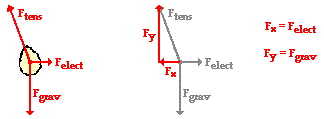
\includegraphics[width=\medgraph,scale=0.01]{frbdy.png}
		%h (here) - same location
		%t (top) - top of page
		%b (bottom) - bottom of page
		%p (page) - on an extra page5
		%! (override) - will force the specified location
		\caption{Free body diagram of a charged sphere suspeded from a string. Photo Credit \cite{physcls} 
		}
		\label{frbdy}
	\end{figure}

	\indent Provided the mass of the sphere, the force due to gravity this object experiences can be computed. As the tension force has both an x and y component, these two directions can be related by the angle $\theta$, specifically, the angle at which the sphere attached to the rope is suspended. As observable in the diagram rendered in Figure \ref{frbdy}, the horizontal (x) component of this tension force corresponds to the electrostatic force of the sphere. Given the distance from the other sphere and the length of the string, we can compute the electrostatic force acting on each sphere -- which is surprising since we do not need to know the charge on either sphere.\\
	
	\indent However, the electrostatic force is not the only thing which can be calculated using couloumb's law. We can also calculate the electric field $\vec{E}$ surrounding a point particle, which is defined as\cite{electricfield}:
	\begin{align}
	\vec{E} = \frac{\vec{F^E_t}}{q_t} = \frac{kq}{r^2}\hat{r}
	\end{align} 
	where $q_t$ is a test-charge present at a distance $r$ from the point-particle with charge $q$ creating the electric field. Note that the equation for an electric field does not depend on any charge but the charge of the particle creating the field, and it is therefore a measure of how that particle interacts with $any$ charged or polarized object.
	
	\indent However, Coulomb's law can only calculate the electrostatic force acting between two point particles. In order to calculate the electric field generated by extended objects, we must use different methods than a straight-forward application of Coulomb's law.	
	
	\section{Electric Field Due to a Line of Charge}
	\indent In this virtual lab, we wanted to measure the electrostatic force a charged rod exerts on a hanging test charge. (a hanging charged sphere). In order to measure the electric field strength created by the rod at different radii, we hanged a ball with 35nC of charge and measured how much the ball was displaced when a charged rod of length 0.7104m was brought near it. Given the displacement of the ball and the ball's mass, we were able to determine the electric force acting on the ball. Given the charge of the ball, we were able to determine what the electric field magnitude due to the rod at the position of the ball. The results of our measurements are shown in Figure \ref{Fld}.\\
	
	\begin{figure}[h]
		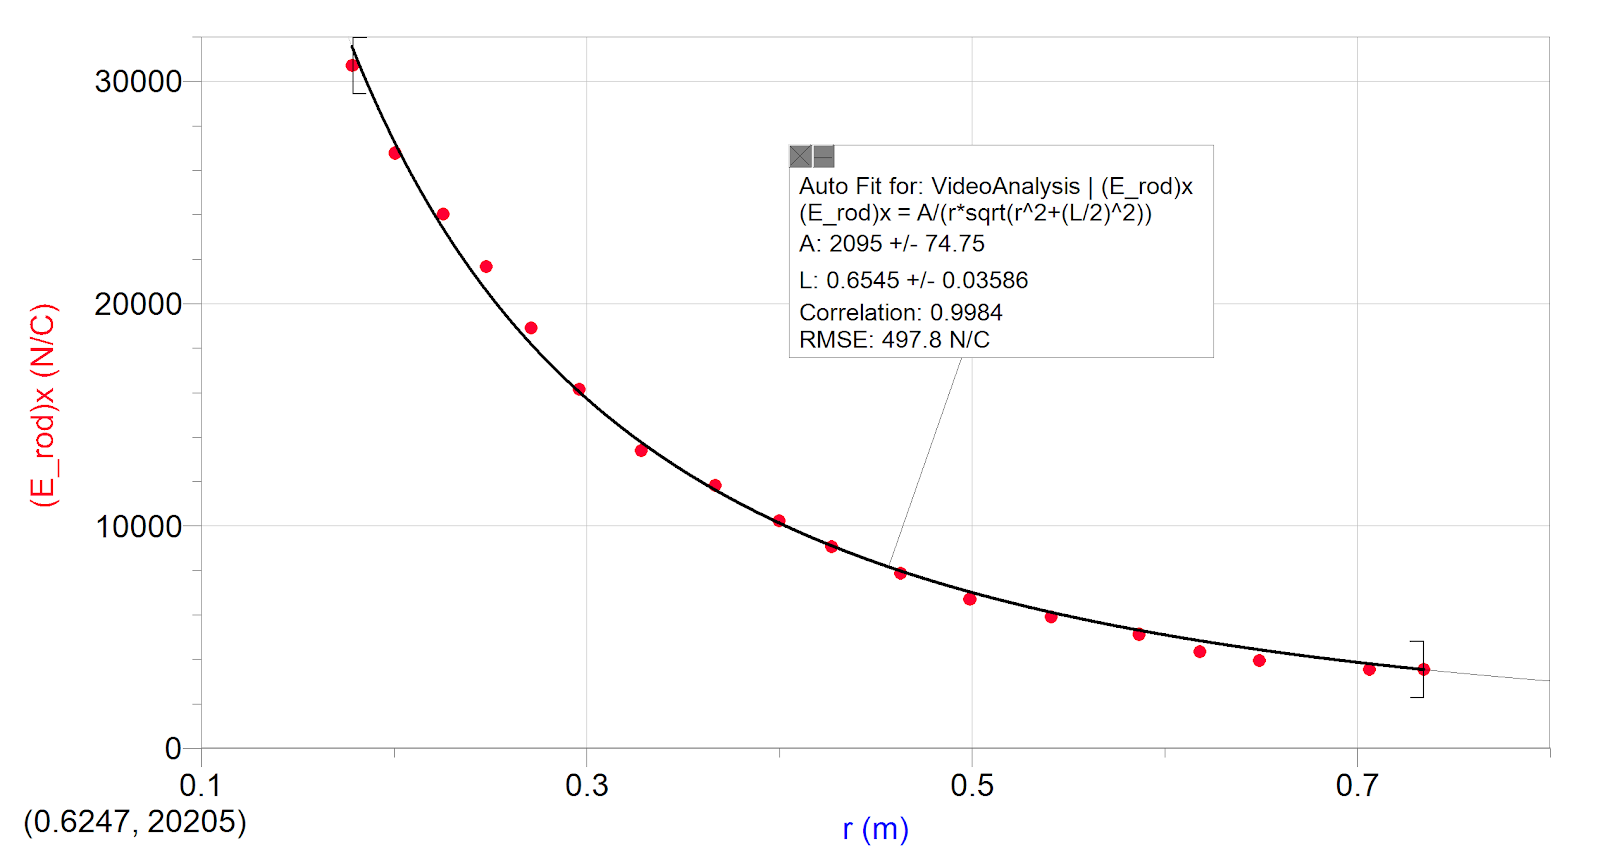
\includegraphics[width=\medgraph,scale=0.01]{FieldStrength.png}
		%h (here) - same location
		%t (top) - top of page
		%b (bottom) - bottom of page
		%p (page) - on an extra page5
		%! (override) - will force the specified location
		\caption{The electric field of the virtual rod (N/C) plotted against its distance from the charged sphere (m). 
		}
		\label{Fld}
	\end{figure}
	
	\indent Note that the line of best fit is given by :
	\begin{align*}
	x=\frac{A}{r\sqrt{r^2+(L/2)^2}	}
	\end{align*}
	where $A\approx 2095$, L is the length of the rod and r is the distance between the rod and the ball.
	
	\indent We are given that $A\approx kQ_{rod}$. From this we can derive the charge present on the rod. We predict that the rod will likely have a charge magnitude that is significantly greater than the hanging charge, since we obtained charges greater than 35nC by friction in previous experiments. To obtain the exact value of the charge on the rod, we compute:
	\begin{align*}
	2095\:\text{Nm}^2/C &\approx kQ_{rod}\\
	\frac{2095\:\text{Nm}^2/C}{k}&\approx Q_{rod}\\
	Q_{rod}&\approx 0.233\mu\text{C}
	\end{align*}
	
	\indent And indeed we see that $Q_{rod}>Q_{ball}$. We would also like a mathematical derivation of the equation for the line of best fit, so that we may better understand the electric field generated by a thin rod.\\
	
	\indent Since we only know how to derive the electric field generated by a point-particle, we orient the rod such that it lies on the y-axis on an x-y plain and then divide the rod into infinitesimally small pieces of length $dy$, such that each piece acts like a point-particle. Then, the charge of that particle would be $dy\cdot \lambda$, where $\lambda = Q_{rod}/L$ is the charge density of the rod.\\
	
	\indent With this information, we can conclude from our definition of an Electric Field for a point particle at a distance R, that: 
	\begin{align*}
	 dE = k\frac{dQ}{R^2} = \frac{k\lambda dy}{R^2}
	\end{align*}
	where $dE$ is an infinitesimal piece of the electric field produced by the rod and $dQ$ is the corresponding charge of the piece of the rod creating the field.\\
	
	\indent Now note that due to symmetry, the field at a particle placed at the midpoint of the rod (as the ball was placed) would have no y-component, since the repulsive force coming from the top and bottom parts of the rod would cancel in the y-direction. Thus, the only components would be in the x-direction. Therefore we can compute:
	\begin{align*}
	E &= 2\int_0^{L/2}\cos(\theta)\frac{k\lambda dy}{R^2}\\
	&=2k\lambda \int_0^{L/2} \cos(\theta)\frac{dy}{R^2}\\
	&=2k\lambda \int_0^{L/2} \cos(\theta)\frac{dy}{r^2+y^2} &&\text{Pythagorean Theorem}\\
	&let\:\:\:y=r\tan(\theta)\\
	&\:\:\: \:\:\:dy = r\sec^2(\theta)d\theta\\
	\implies E&=2k\lambda \int_{\theta_0}^{\theta_1} cos(\theta) \frac{r\sec^2(\theta)d\theta}{r^2\sec^2(\theta)}\\
	E&=\frac{2k\lambda}{r} \int_{\theta_0}^{\theta_1} cos(\theta) \\
	&=\frac{2k\lambda}{r}\sin(\theta_1)\\
	&=\frac{k\lambda}{r}\cdot\frac{L}{\sqrt{r^2+(L/2)^2}}\\
	E&= \frac{kQ_{rod}}{r\sqrt{r^2(L/2)^2}}\\
	\vec{E} &=  \frac{kQ_{rod}}{r\sqrt{r^2(L/2)^2}}\hat{i}
	\end{align*}
	Where the last step is justified since the field will have non-zero magnitude only along the $\hat{i}$ direction (positive x-axis).
	And thus we have derived the same formula determined empirically for the electric field generated by a thin rod.
	
	\section{Discharge Rate}
	In this virtual lab, we wanted to measure the rate of electrical discharge of an object. To do so, we derived equations needed to determine the amount of charge on two balls as a function of their separation.\\
	
	\indent Figure \ref{scn} shows the free-body diagram used to visualize the derivation of the electrostatic force acting one of the balls. The derivation is as follows: In a state of equilibrium, we require that the vector sum of all the forces be 0. Also, note that the electrostatic force $\vec{F^{coul}}$ is horizontal and thus points only in the $\hat{i}$ direction. Therefore, the sum of the gravitational force $\vec{F^{grav}}$ and the tension force $\vec{F^{tens}}$ in the $\hat{j}$ direction must be zero. So for $R$ = distance between the two balls, $L$ = length of the strings, $m$ = mass of each ball, and $g$ = 9.8m/$\text{s}^2$ we can derive:
	\begin{align*}
		\vec{F^{tens}} \cdot \hat{j} &= mg\\
		\cos(\theta)F^{tens} &= mg\\
		F^{tens} &= \frac{mg}{\cos(\theta)}\\
		\implies F^{coul} &= F^{tens}\cdot \hat{i} = \frac{mg}{\cos(\theta)}\sin(\theta)\\
		&=mg\tan(\theta)\\
		F^{coul} &\approx \frac{mgR}{2L}
	\end{align*}
	where the last step is justified since for $L>>R/2$ and $\theta << 0$, $tan(\theta) \approx \sin(\theta) = (R/2)/L$.\\
	
	\indent Also note that R can be given by $R = |X_1-X_2|$ where $X_1$ is the location of ball 1 and $X_2$ is the location of ball 2. Using these formulas, we were able to obtain the data in Figures \ref{loc}-\ref{Charge}.\\
	 
		\begin{figure}[h]
		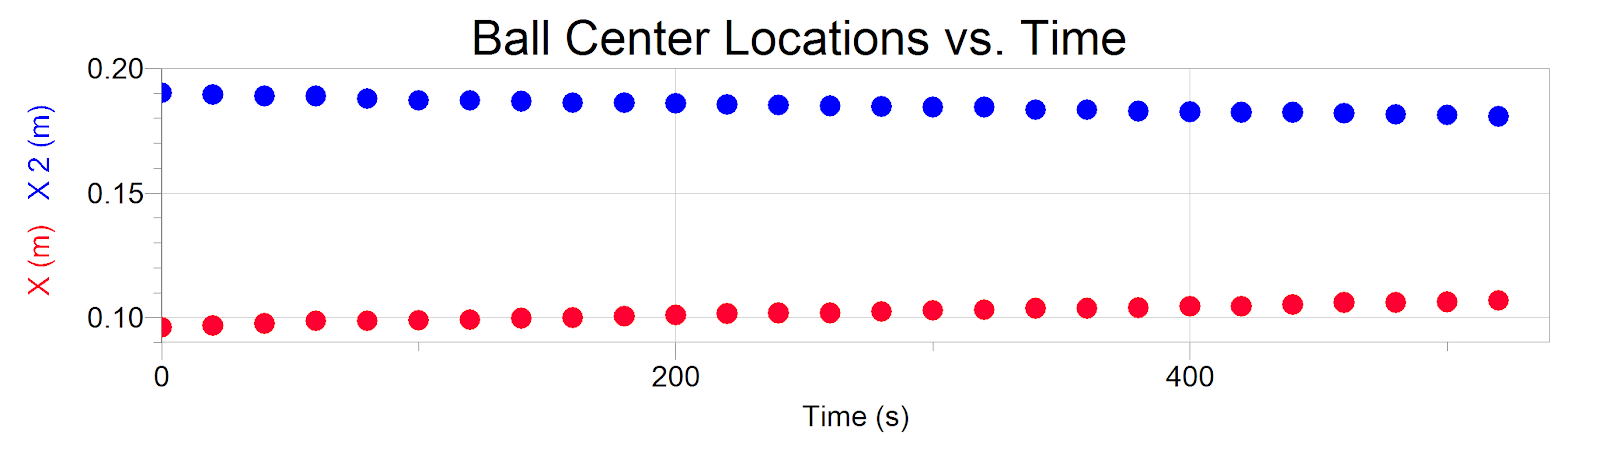
\includegraphics[width=\linewidth,scale=0.01]{LocvTime.png}
		%h (here) - same location
		%t (top) - top of page
		%b (bottom) - bottom of page
		%p (page) - on an extra page5
		%! (override) - will force the specified location
		\caption{The position of the center location of both ball 1 and ball 2, denoted as X (m) and X 2 (m) respectively, versus time (s).}
		\label{loc}
	\end{figure}
\begin{figure}[h]
	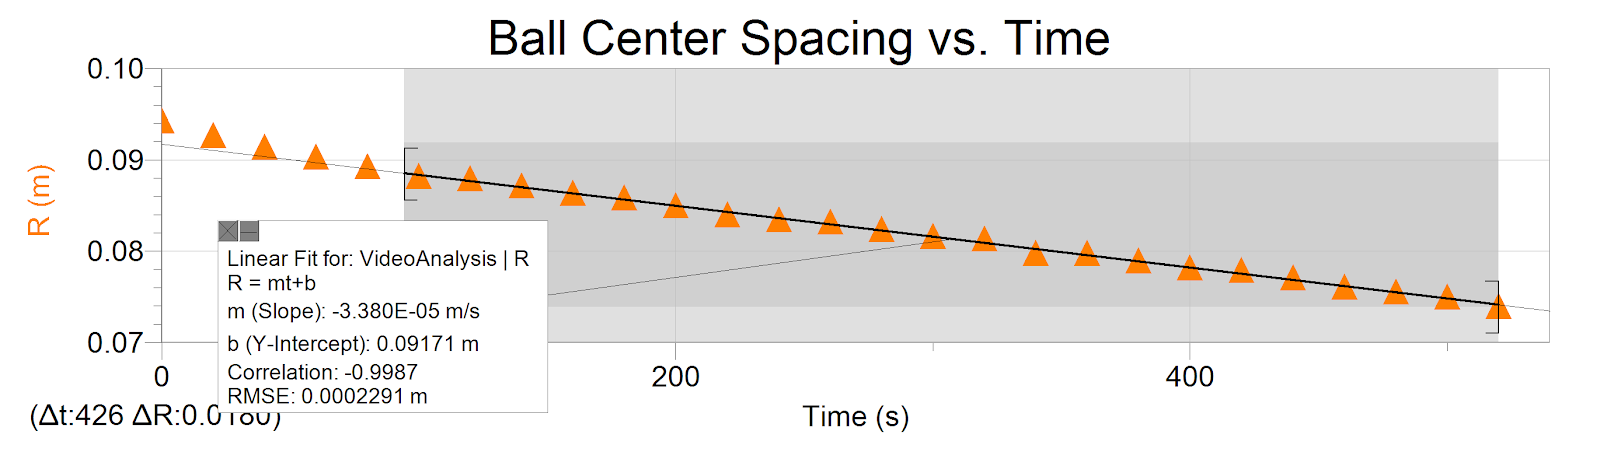
\includegraphics[width=\linewidth,scale=0.01]{SpacevTime.png}
	%h (here) - same location
	%t (top) - top of page
	%b (bottom) - bottom of page
	%p (page) - on an extra page5
	%! (override) - will force the specified location
	\caption{The separation of the centers of both ball 1 and ball 2, denoted as R (m), versus time (s).}
	\label{Space}
\end{figure}

\begin{figure}[h]
	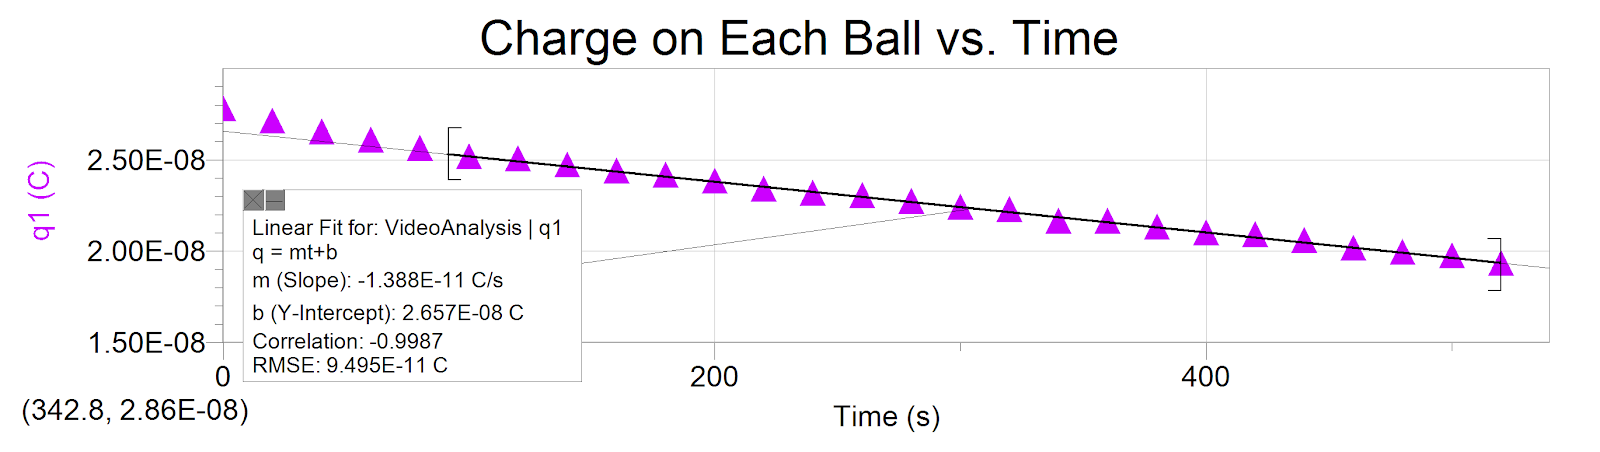
\includegraphics[width=\linewidth,scale=0.01]{ChargevTime.png}
	%h (here) - same location
	%t (top) - top of page
	%b (bottom) - bottom of page
	%p (page) - on an extra page5
	%! (override) - will force the specified location
	\caption{The charge on ball 1 (C) versus time (s). Given that the mass and charge of the two balls were nearly identical, only ball 1 was used for analysis.}
	\label{Charge}
	
\end{figure}

	\begin{figure}[h]
	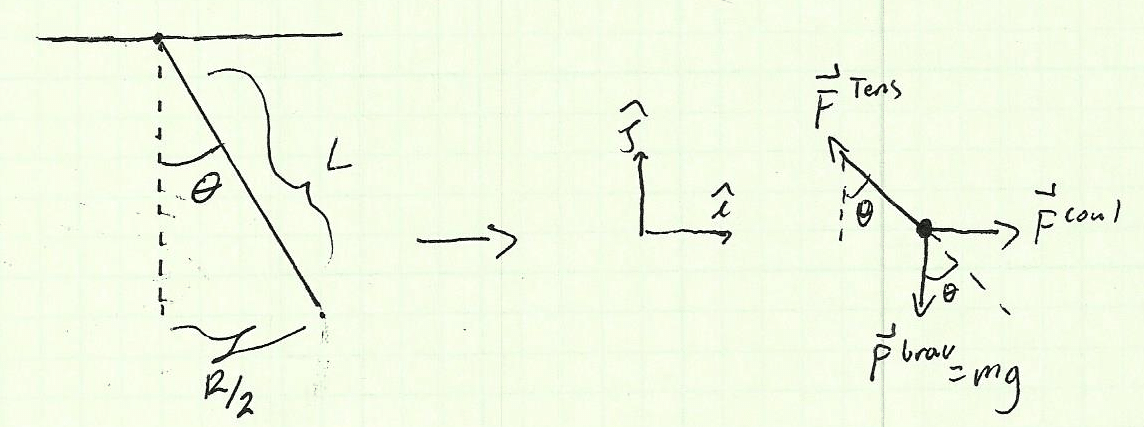
\includegraphics[width=\linewidth,scale=0.01]{scan.png}
	%h (here) - same location
	%t (top) - top of page
	%b (bottom) - bottom of page
	%p (page) - on an extra page5
	%! (override) - will force the specified location
	\caption{Free-body diagram of one of the charged balls suspended from a string}
	\label{scn}
\end{figure}


\indent The linear regression line given in Figure \ref{Space} allows us to predict the time at which the two balls will touch. Given that the distance R at any time $t$ is given by $R = -3.380\times10^{-5}t + 0.09171$, we can predict that $R=0 \implies t \approx 2713$s which corresponds approximately 45 minutes.\\

\indent Figure \ref{Charge} shows that the charge on each ball also decreases with time. This result is not surprising, since the charged balls come closer together with time, which indicates that the system is not in equilibrium (if it was, we would observe that the balls eventually remain stationary without touching). The most likely explanation for the loss of charge on each ball is that their charge is lost to the moisture in the air.\\

\indent However, note that the charge initially decreases faster than the regression line (prior to 100s). This indicates that there may be another drain for the charge which is significant only when the charges on a given ball is very large. This additional discharge may be due to the non-conducting string. While the charge is very high, the difference in charge between the ball and the string may cause electrons to move along the surface of the string, which would cause the more rapid charge loss that was observed when $t\le 100$s. 

\section{Conclusion}
\newpage
\printbibliography
\end{document}